% Chapter Title Page
\clearpage
\thispagestyle{empty} 
\begin{center}
    \vspace*{\fill} 
    \Huge \textbf{Chapter 5} \\
    \Huge \textbf{Symmetric Encryption} 
    \vspace*{\fill}
\end{center}
\clearpage
\chapter{Symmetric Encryption}

\section{Definition}
Symmetric encryption, also known as secret-key encryption, is a cryptographic scheme where the same key is used for both encryption and decryption.

\section{Ingredients of Symmetric Encryption}
\begin{figure}
    \centering
    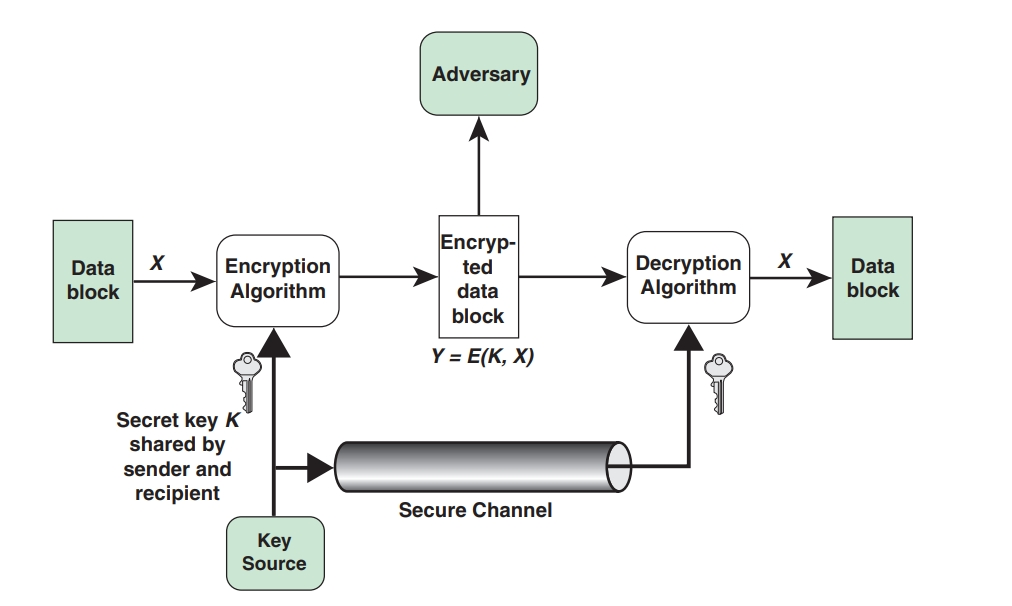
\includegraphics[width=1\linewidth]{Data_Privacy_and_Cryptography/Figures/model of symmetric crypto.jpeg}
    \caption{Model of Symmetric Cryptosystem}
    \label{fig:enter-label}
\end{figure}
\begin{itemize}
    \item \textbf{Plaintext:} The original message or data block that is input into the encryption algorithm.
    \item \textbf{Encryption Algorithm:} The algorithm that performs various substitutions and transformations on the plaintext using the secret key.
    \item \textbf{Secret Key:} An input to the encryption algorithm; the exact substitutions and transformations depend on this key.
    \item \textbf{Ciphertext:} The scrambled message produced as output. It depends on both the plaintext and the secret key. Different keys produce different ciphertexts for the same plaintext.
    \item \textbf{Decryption Algorithm:} The inverse of the encryption algorithm; it uses the ciphertext and the secret key to reproduce the original plaintext.
\end{itemize}

\section{Requirements for Secure Symmetric Encryption}

\begin{itemize}
    \item \textbf{Strong Encryption Algorithm:} 
    \begin{itemize}
        \item The algorithm should be such that an opponent, even with access to the algorithm and multiple ciphertexts, cannot decipher the ciphertext or determine the key.
        \item Ideally, the opponent should not be able to decrypt the ciphertext or discover the key even if they possess multiple ciphertext-plaintext pairs.
    \end{itemize}
    \item \textbf{Secure Key Distribution:} 
    \begin{itemize}
        \item The sender and receiver must obtain copies of the secret key in a secure manner and must keep the key secure.
        \item If an opponent discovers the key, they can read all communications encrypted with that key.
    \end{itemize}
\end{itemize}


\section{Key Generation and Distribution}

A key generation algorithm typically generates a random number and derives a secret key from it.

For two parties to communicate, key distribution can occur through various methods:
\begin{itemize}
    \item One party generates the key and securely transfers it to the other party.
    \item A secure key exchange protocol enables both parties to jointly generate a key known only to them.
    \item A third party generates the key and securely transfers it to the two communicating parties.
\end{itemize}

\section{Potential Adversary Attacks}

\begin{itemize}
    \item \textbf{Cryptanalysis:} 
    \begin{itemize}
        \item Relies on the nature of the algorithm and knowledge of the plaintext or sample plaintext/ciphertext pairs.
        \item  It attempts to deduce the key or specific plaintext.
        \item If successful, all past and future messages encrypted with that key are compromised.
    \end{itemize}
     
    \item \textbf{Brute-Force Attack:}
    \begin{itemize}
        \item  Involves trying every possible key on a piece of ciphertext until an intelligible translation into plaintext is found.
        \item  On average, half of all possible keys must be tried to achieve success.
        \item A secure symmetric encryption scheme requires an algorithm resistant to cryptanalysis and a key of sufficient length to defeat brute-force attacks.
   
    \end{itemize}
\end{itemize}



